\section{Quantum Receiver}
    The problem of quantum receiver is one of the most important
    aspects of quantum communication. As in classical communication, the ability to 
    distinguish between two or more states in presence of noise can be decisive in order to determine
    the performance of the communication system. The problem of the receiver can be, therefor, reformulated
    as a problem of discrimination between two states.
    However, differently from the classical situation,
    the discrimination can be done using a custom-designed quantum discriminator, overcoming
    the classical physics limits.

    \subsection{Binary case}
    The problem of discrimination between two quantum states is realized, as every measurement
    process \ref{post:2}, using an operator or a set of operators.
    If the state of the system is unknown, as shown in figure \ref{fig:2.2}, there are two hypotheses
    about the state $\Operator{\varXi}$ (the problem is easly generalizable for $M$ different states),
    given by:
    \begin{equation}\begin{split}
        H_0 &: \Operator{\varXi}=\Operator{\varXi}_0\\
        H_1 &: \Operator{\varXi}=\Operator{\varXi}_1
        \label{eq:binHyp}
    \end{split}\end{equation}
    It is necessary a set of two positive-definites operator (POVM)
    \begin{equation}
        \mathcal{P}=\{\Operator{\varPi}_0,\Operator{\varPi}_1\}
    \end{equation}
    for the discrimination process, and the probability that the hypothesis $H_j$ is choosen
    if $H_k$ is the right choose is given by \cite{tesiGuerrini}:
    \begin{equation}
        \mathbb{P}\{H_j|H_k\}=\tr{\Operator{\varXi}_k\Operator{\varPi}_j}.
    \end{equation}
    The distribution error probability (DEP) in the discrimination process, if $p_0$ and $p_1$ are 
    respectively the probabilty of symbols $0$ and $1$, is so given by
    \begin{equation}
        P_e=1-\left(p_0 \tr{\Operator{\varXi}_0\Operator{\varPi}_0}+p_1 \tr{\Operator{\varXi}_1\Operator{\varPi}_1}\right).
    \end{equation}

    \subsection{Optimal binary receiver}
    \begin{figure}[t]
        \begin{center}
            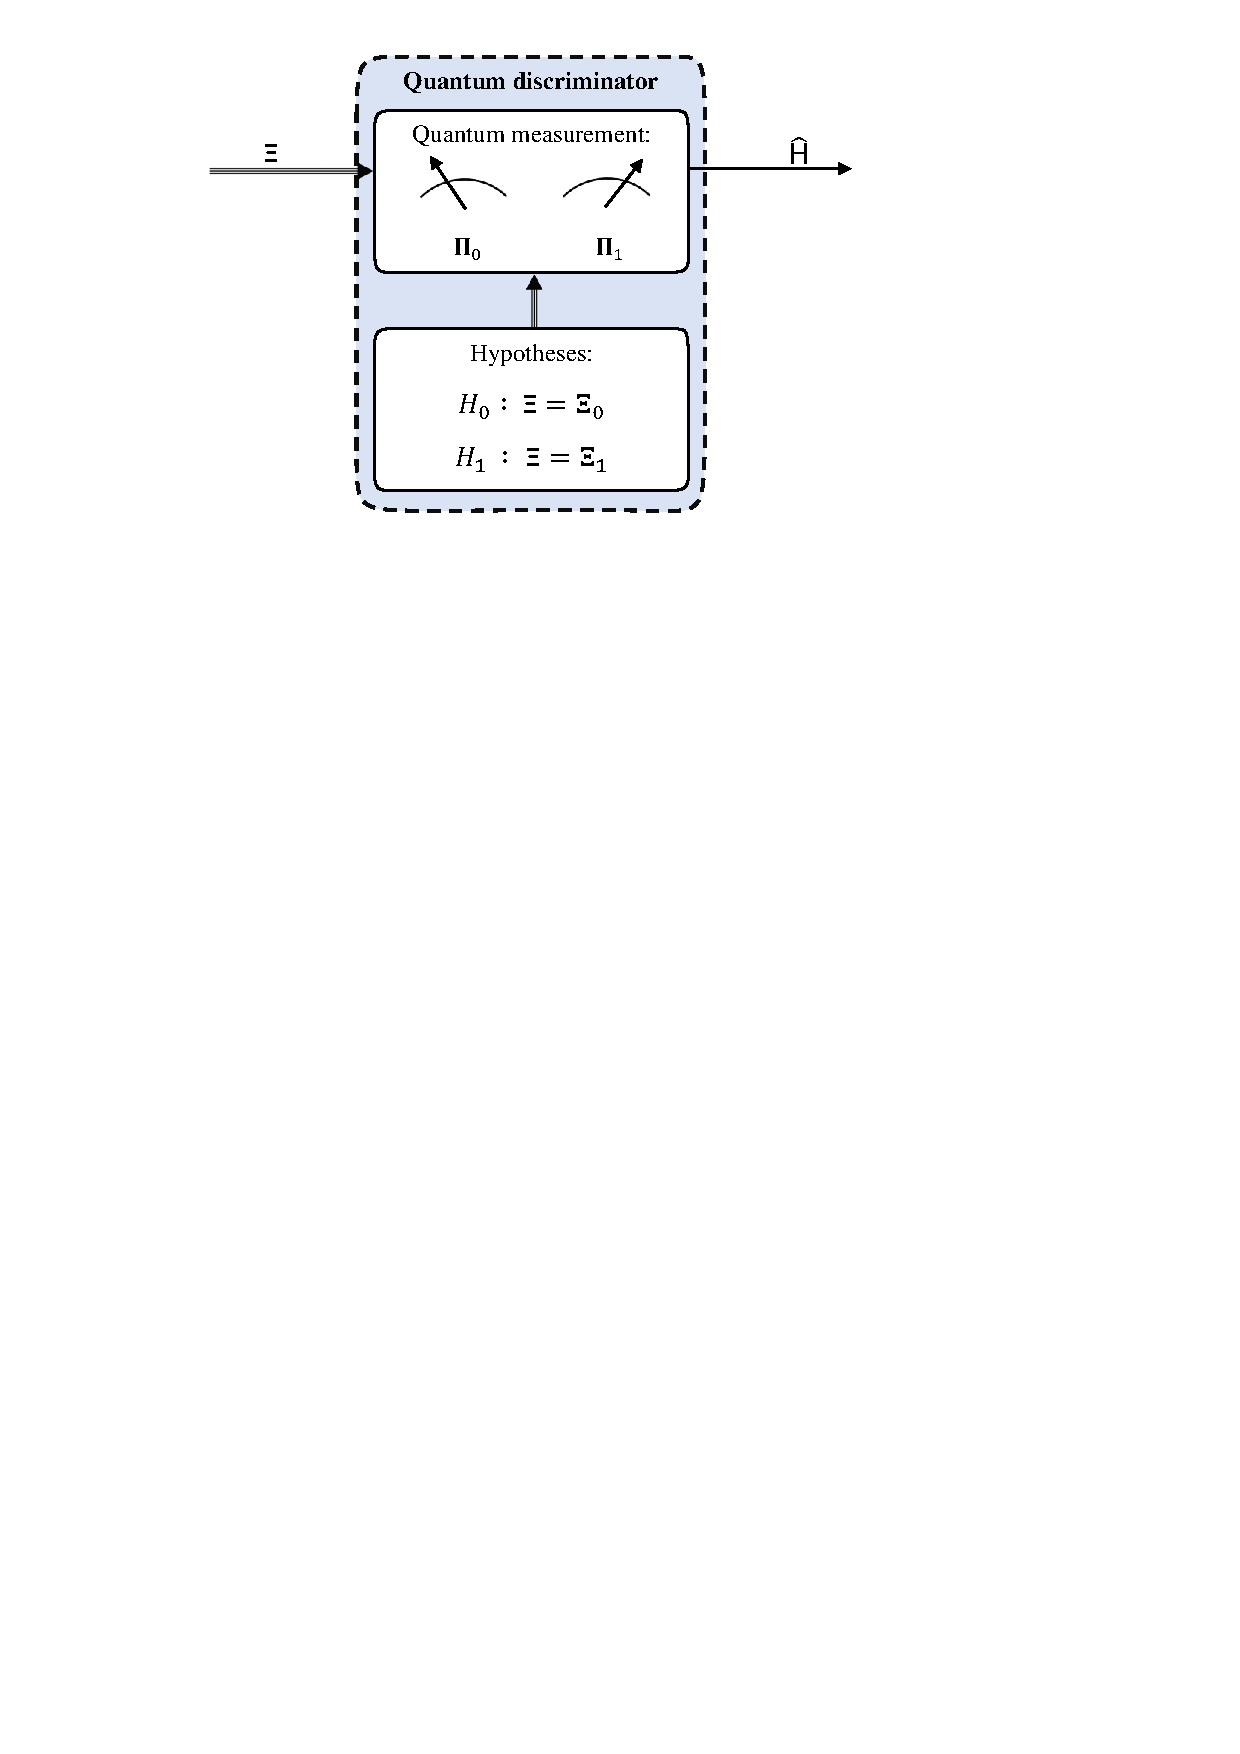
\includegraphics[width=0.75\textwidth]{fig2.2.pdf}
            \caption{Binary quantum state discriminator.}
            \label{fig:2.2}
        \end{center}
    \end{figure}
    The issue of finding the optimal POVM that minimizes the DEP was exhaustively discuss  by Helstrom in 
    \cite{helstrom3,helstrom4}. The minimum distribution error probability (MDEP) for a binary 
    communication system is given by the well-known Helstrom bound
    \begin{equation}
        \breve{P}_e = \frac{1}{2} \left(1-\norm{p_1 \Operator{\varXi}_1 - p_0 \Operator{\varXi}_0}_1 \right),
        \label{eq:HelstromBound}
    \end{equation}
    where $p_0,\ p_1$ are the probability that the states $\Operator{\varXi}_0,\ \Operator{\varXi}_1$ are trasmitted
    and the operator $\norm{\cdot}_1$ represents the trace norm. 
    The MDEP \ref{eq:HelstromBound} is obtained with the POVM defined as
    \begin{equation}
        \breve{\Operator{\varPi}}_0 = \sum_{\substack{i \\ \lambda_i<0}} \ket*{\lambda_i}\bra*{\lambda_i},
    \end{equation}
    \begin{equation*}
        \breve{\Operator{\varPi}}_1 = 1-\breve{\Operator{\varPi}}_0 = 
        \sum_{\substack{i \\ \lambda_i \geq 0}} \ket*{\lambda_i}\bra*{\lambda_i};
    \end{equation*}
    where $\ket*{\lambda_i}$ is the eigenvector of $p_1 \Operator{\varXi}_1 - p_0 \Operator{\varXi}_0$ associated to 
    the eigenvalue $\lambda_i$.
    For pure states, i.e $\Operator{\varXi}_0 = \ket*{\psi_0}\bra*{\psi_0}$ and $\Operator{\varXi}_1 = \ket*{\psi_1}
    \bra*{\psi_1}$, the equation \ref{eq:HelstromBound} begin
    \begin{equation}
        \breve{P}_e = \frac{1}{2} \left(1- \sqrt{1-4 p_0 p_1 \absolutevalue{\braket{\psi_0}{\psi_1}}^2}
        \right).
        \label{eq:HelstromBPure}
    \end{equation}
    It is possible to observe that, for pure states, the MDEP is equal to $0$ if $\braket{\psi_0}{\psi_1}$,
    that is $\ket{\psi_0}$ and $\ket{\psi_1}$ are orthogonal states.